\appendix


\section{Appendiks - Programmeringselementer i \texttt{FB}}\label{app:FB-elementer}  

Utfyllende beskrivelser og eksempler på bruk finnes i hjelpesystemet: Velg det aktuelle
programmeringselementet og trykk “\verb|F1|” så kommer det fram mange nyttige tips.

\begin{center}
 \resizebox{\columnwidth}{!}{\begin{tabular}{|c| c| m{11cm}| } 
 \hline
 \textbf{Symbol} & \textbf{Betegnelse} & \textbf{Beskrivelse}  \\ 
 \toprule
 
 
   \begin{tikzpicture}[baseline=0]
    \draw (-1.5,-0.75) rectangle (1.5,0.75) ;
    \draw (-2,-0.4) -- (-1.5,-0.4) ;
    \draw (-2,0.1) -- (-1.5,0.1) ;
    \draw (1.5,-0.4) -- (2,-0.4) ;
    \draw (-0.1, 0.6) node [anchor=north west][inner sep=0.75pt]   [align=left] {\texttt{\&}};

        \addvmargin{2mm}
  \end{tikzpicture}    & \texttt{AND} & \makecell{Beregner logisk “\texttt{AND}” av inngangene.
Hvis alle inngangene har \\ verdien “\texttt{TRUE}” blir utgangen også
“\texttt{TRUE}”. I motsatt fall blir \\ utgangen “\texttt{FALSE}”.}\\ 
 \hline
 \begin{tikzpicture}[baseline=0]
    \draw (-1.5,-0.75) rectangle (1.5,0.75) ;
    \draw (-2,-0.4) -- (-1.5,-0.4) ;
    \draw (-2,0.1) -- (-1.5,0.1) ;
    \draw (1.5,-0.4) -- (2,-0.4) ;
    \draw (-0.35, 0.6) node [anchor=north west][inner sep=0.75pt]   [align=left] {\texttt{>=1}};

        \addvmargin{2mm}
  \end{tikzpicture} & \texttt{OR}  & \makecell{Beregner logisk “\texttt{OR}” av inngangene.
Hvis minst en av\\ inngangene har verdien “\texttt{TRUE}” blir utgangen
også “\texttt{TRUE}”. \\I motsatt fall blir utgangen “\texttt{FALSE}”.}\\ 


 \hline
 \begin{tikzpicture}[baseline=0]
    \draw (-1.5,-0.75) rectangle (1.5,0.75) ;
    \draw (-2,-0.4) -- (-1.5,-0.4) ;
    \draw (-2,0.1) -- (-1.5,0.1) ;
    \draw (1.5,-0.4) -- (2,-0.4) ;
    \draw (-0.35, 0.6) node [anchor=north west][inner sep=0.75pt]   [align=left] {\texttt{XOR}};

        \addvmargin{2mm}
  \end{tikzpicture}  & \texttt{Exclusive OR} & \makecell{Beregner logisk “\texttt{XOR}” av de to inngangene.
Hvis en og bare \\ en av inngangene har verdien “\texttt{TRUE}” blir
utgangen “\texttt{TRUE}”. I \\ motsatt fall blir utgangen “\texttt{FALSE}”.}\\ 


 \hline
\begin{tikzpicture}[baseline=0]
    \draw (0,-0.75) -- (0,0.75) ;
    \draw (-0.19,0) circle (5pt);
    \draw (-0.7,0) -- (-0.375,0) ;

        \addvmargin{2mm}
  \end{tikzpicture}  & \texttt{Inverter} & \makecell{Settes på binære innganger for å invertere disse.}\\ 
 \hline
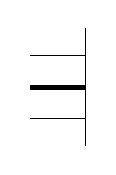
\begin{tikzpicture}[baseline=0]
    \draw (0,-0.75) -- (0,0.75) ;
    \draw [line width=0.6mm] (-0.7,0) -- (-0,0) ;
    \draw (-0.7,0.4) -- (-0,0.4) ;
    \draw (-0.7,-0.4) -- (-0,-0.4) ;

        \addvmargin{2mm}
  \end{tikzpicture}  & \texttt{Binary input} & \makecell{Brukes hvis det trengs flere enn to innganger til en \texttt{OR}- eller \\
\texttt{AND}-port.}\\ 
 \hline
 \begin{tikzpicture}[baseline=0]
    \draw (-1.2,-0) -- (1.2,0) ;
    \draw (-.3,0) -- (-.3,-1) ;
    \draw (-.3,-1) -- (1,-1) ;

        \addvmargin{4.5mm}
  \end{tikzpicture} & \centered{ \\ \\ \texttt{Branching}} & \makecell{\\ Brukes hvis samme signal skal brukes som inngang til flere \\ andre
bokser.}\\ 


 \hline
  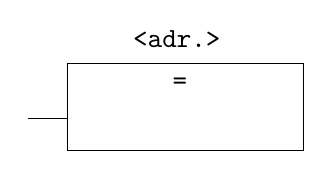
\begin{tikzpicture}[baseline=0]
    \draw (-1.5,-0.6) rectangle (1.5,0.5) ;
    \draw (-2,-0.2) -- (-1.5,-0.2) ;
    
    \draw (-0.7, 0.95) node [anchor=north west][inner sep=0.75pt]   [align=left] {\texttt{<adr.>}};
    \draw (-0.2, 0.35) node [anchor=north west][inner sep=0.75pt]   [align=left] {\texttt{=}};

        \addvmargin{2mm}
  \end{tikzpicture}  & \texttt{Assign output} & Setter utgang (med spesifiserte adresse) lik verdien til inngang.\\ 
 \hline
  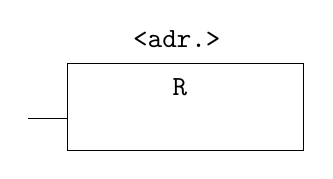
\begin{tikzpicture}[baseline=0]
    \draw (-1.5,-0.6) rectangle (1.5,0.5) ;
    \draw (-2,-0.2) -- (-1.5,-0.2) ;
    
    \draw (-0.7, 0.95) node [anchor=north west][inner sep=0.75pt]   [align=left] {\texttt{<adr.>}};
    \draw (-0.2, 0.35) node [anchor=north west][inner sep=0.75pt]   [align=left] {\texttt{R}};

        \addvmargin{2mm}
  \end{tikzpicture} & \texttt{Reset output} & \makecell{Hvis inngangen er “\texttt{TRUE}”, resettes den spesifiserte utgangen \\ til \texttt{0}.
Hvis inngangen er “\texttt{FALSE}”, beholder utgangen sin gamle \\ verdi.} \\ 
 \hline
  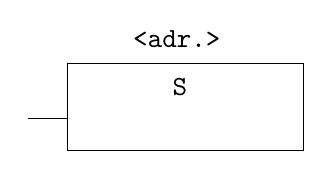
\begin{tikzpicture}[baseline=0]
    \draw (-1.5,-0.6) rectangle (1.5,0.5) ;
    \draw (-2,-0.2) -- (-1.5,-0.2) ;
    
    \draw (-0.7, 0.95) node [anchor=north west][inner sep=0.75pt]   [align=left] {\texttt{<adr.>}};
    \draw (-0.2, 0.35) node [anchor=north west][inner sep=0.75pt]   [align=left] {\texttt{S}};

        \addvmargin{2mm}
  \end{tikzpicture} & \texttt{Set output} & \makecell{Hvis inngangen er “\texttt{TRUE}”, settes den spesifiserte utgangen til \\ \texttt{1}.
Hvis inngangen er “\texttt{FALSE}”, beholder utgangen sin gamle \\ verdi.}\\ 
 \hline

\end{tabular}}
\end{center}

\begin{center}
 \resizebox{\columnwidth}{!}{\begin{tabular}{|c| c| m{11cm}| } 
 \hline
 \textbf{Symbol} & \textbf{Betegnelse} & \textbf{Beskrivelse}  \\ 
 \toprule
 
  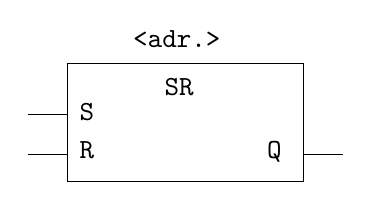
\begin{tikzpicture}[baseline=0]
    \draw (-1.5,-0.75) rectangle (1.5,0.75) ;
    \draw (-2,-0.4) -- (-1.5,-0.4) ;
    \draw (-2,0.1) -- (-1.5,0.1) ;
    \draw (1.5,-0.4) -- (2,-0.4) ;
    
    \draw (-0.7, 1.2) node [anchor=north west][inner sep=0.75pt]   [align=left]  {\texttt{<adr.>}};
    \draw (-0.3, 0.6) node [anchor=north west][inner sep=0.75pt]   [align=left] {\texttt{SR}};
    
    \draw (-1.38, 0.28) node [anchor=north west][inner sep=0.75pt]   [align=left] {\texttt{S}};
    \draw (-1.38, -0.2) node [anchor=north west][inner sep=0.75pt]   [align=left] {\texttt{R}};
    
    \draw (1, -0.2) node [anchor=north west][inner sep=0.75pt]   [align=left] {\texttt{Q}};



        \addvmargin{2mm}
  \end{tikzpicture}  & \texttt{SR flip flop} & \makecell{Hvis inngang \texttt{S} er “\texttt{TRUE}”, settes den spesifiserte utgangen til \\ \texttt{1}.
Hvis inngang \texttt{R} er “\texttt{TRUE}”, resettes den spesifiserte utgangen \\ til \texttt{0}.
Hvis både \texttt{S} og \texttt{R} er “\texttt{FALSE}”, beholder utgangen sin gamle \\ verdi.}\\ 
 \hline
 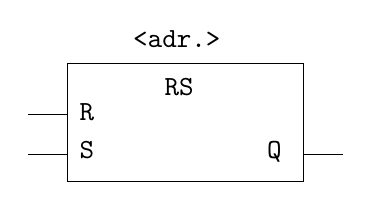
\begin{tikzpicture}[baseline=0]
    \draw (-1.5,-0.75) rectangle (1.5,0.75) ;
    \draw (-2,-0.4) -- (-1.5,-0.4) ;
    \draw (-2,0.1) -- (-1.5,0.1) ;
    \draw (1.5,-0.4) -- (2,-0.4) ;
    
    \draw (-0.7, 1.2) node [anchor=north west][inner sep=0.75pt]   [align=left]  {\texttt{<adr.>}};
    \draw (-0.3, 0.6) node [anchor=north west][inner sep=0.75pt]   [align=left] {\texttt{RS}};
    
    \draw (-1.38, 0.28) node [anchor=north west][inner sep=0.75pt]   [align=left] {\texttt{R}};
    \draw (-1.38, -0.2) node [anchor=north west][inner sep=0.75pt]   [align=left] {\texttt{S}};
    
    \draw (1, -0.2) node [anchor=north west][inner sep=0.75pt]   [align=left] {\texttt{Q}};



        \addvmargin{2mm}
  \end{tikzpicture} & \texttt{RS flip flop}  & \makecell{Samme som \texttt{SR}-vippe. Den eneste forskjellen er hvis både \texttt{S} og \\ \texttt{R}
er “\texttt{TRUE}”. Da vil den inngangen som står nederst vinne over \\ den
som står øverst. Dvs. at \texttt{SR}-vippa vil bli resatt hvis begge \\
inngangene er “\texttt{TRUE}”.}\\ 
 \hline
 
 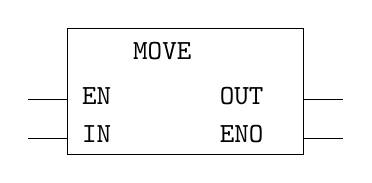
\begin{tikzpicture}[baseline=0]
    \draw (-1.5,-.8) rectangle (1.5,.8) ;
    
    \draw (-2,-0.6) -- (-1.5,-0.6) ;
    
    \draw (1.5,-0.6) -- (2,-0.6) ;
    
    \draw (1.5,-0.1) -- (2,-0.1) ;
    
    \draw (-2,-0.1) -- (-1.5,-0.1) ;
    

    \draw (-0.7, 0.65) node [anchor=north west][inner sep=0.75pt]   [align=left] {\texttt{MOVE}};
    
    \draw (-1.35, 0.08) node [anchor=north west][inner sep=0.75pt]   [align=left] {\texttt{EN}};
    \draw (-1.35, -0.4) node [anchor=north west][inner sep=0.75pt]   [align=left] {\texttt{IN}};
    
    \draw (.4, 0.08) node [anchor=north west][inner sep=0.75pt]   [align=left] {\texttt{OUT}};
    \draw (.4, -0.4) node [anchor=north west][inner sep=0.75pt]   [align=left] {\texttt{ENO}};



        \addvmargin{2mm}
  \end{tikzpicture} & \texttt{MOVE} & \makecell{Tilordner verdien på inngangen \texttt{IN} til utgangen \texttt{OUT} så lenge \\
enable \texttt{EN} har verdien “\texttt{TRUE}”.}\\ 
 \hline
 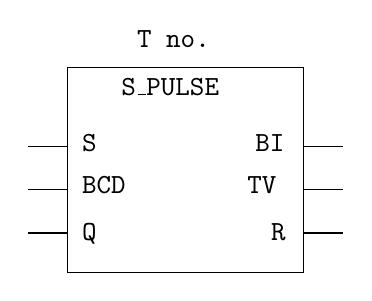
\begin{tikzpicture}[baseline=0]
    \draw (-1.5,-1.3) rectangle (1.5,1.3) ;
    
    \draw (1.5,0.3) -- (2,0.3) ;
    
    \draw (-2,0.3) -- (-1.5,0.3) ;
    
    \draw (-2,-0.25) -- (-1.5,-0.25) ;
    
    \draw (1.5,-0.25) -- (2,-0.25) ;
    
    
    \draw (1.5,-.8) -- (2,-.8) ;
    
    \draw (-2,-.8) -- (-1.5,-.8) ;
  
    
    \draw (-0.65, 1.8) node [anchor=north west][inner sep=0.75pt]   [align=left] {\texttt{T no.}};
    \draw (-0.85, 1.2) node [anchor=north west][inner sep=0.75pt]   [align=left] {\texttt{S\_PULSE}};
    
    \draw (-1.35, 0.48) node [anchor=north west][inner sep=0.75pt]   [align=left] {\texttt{S}};
    \draw (.85, 0.48) node [anchor=north west][inner sep=0.75pt]   [align=left] {\texttt{BI}};
    
    \draw (.75, -0.05) node [anchor=north west][inner sep=0.75pt]   [align=left] {\texttt{TV}};
    \draw (-1.35, -0.05) node [anchor=north west][inner sep=0.75pt]   [align=left] {\texttt{BCD}};
    
    \draw (1.05, -0.65) node [anchor=north west][inner sep=0.75pt]   [align=left] {\texttt{R}};
    \draw (-1.35, -0.65) node [anchor=north west][inner sep=0.75pt]   [align=left] {\texttt{Q}};
        \addvmargin{2mm}
  \end{tikzpicture} & \texttt{Timer} & \makecell{Timeren startes av signalet på inngang \texttt{S} (BOOL). De ulike\\ typene
timere har forskjellige virkemåter med hensyn på når\\ tidtakingen
skal starte og hva verdien på utgangen \texttt{Q} (BOOL) \\skal være. Tiden
timeren skal gå etter den er startet angis på \\ inngang \texttt{TV} med format:
\texttt{S5T\#aH\_bM\_cS\_dMS}
. Se appendiks \ref{app:timer} \\for flere detaljer om timere.}\\ 


 \hline
 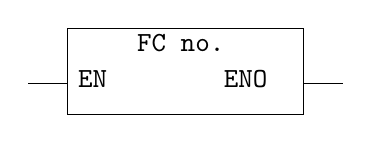
\begin{tikzpicture}[baseline=0]
 \draw (-0.65, 0.35) node [anchor=north west][inner sep=0.75pt]   [align=left] {\texttt{FC no.}};
    \draw ( 0.45, -.1) node [anchor=north west][inner sep=0.75pt]   [align=left] {\texttt{ENO}};
    \draw (-1.4, -.1) node [anchor=north west][inner sep=0.75pt]   [align=left] {\texttt{EN}};
    \draw (-1.5,-0.7) rectangle (1.5,0.4) ;
    \draw (-2,-0.3) -- (-1.5,-0.3) ;
    \draw (1.5,-0.3) -- (2,-0.3) ;

        \addvmargin{3mm}
  \end{tikzpicture} & \centered{\\ Function call} & \makecell{Kall av funksjoner. Husk at det er ikke nok at funksjonene \\ ligger i
prosjektet, det må også gjøres et funksjonskall til dem\\ (typisk med OB1).}\\ 
 \hline
  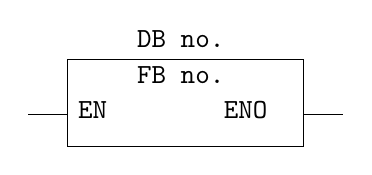
\begin{tikzpicture}[baseline=0]
    \draw (-1.5,-0.7) rectangle (1.5,0.4) ;
    \draw (-2,-0.3) -- (-1.5,-0.3) ;
    \draw (1.5,-0.3) -- (2,-0.3) ;
    
    \draw (-0.65, 0.8) node [anchor=north west][inner sep=0.75pt]   [align=left] {\texttt{DB no.}};
    \draw (-0.65, 0.35) node [anchor=north west][inner sep=0.75pt]   [align=left] {\texttt{FB no.}};
    
    \draw ( 0.45, -.1) node [anchor=north west][inner sep=0.75pt]   [align=left] {\texttt{ENO}};
    \draw (-1.4, -.1) node [anchor=north west][inner sep=0.75pt]   [align=left] {\texttt{EN}};

        \addvmargin{2mm}
  \end{tikzpicture}& Functionblock call & Ved kall av funksjonsblokker hører det alltid med en datablokk. \\ 
 \hline
 

\end{tabular}}
\end{center}

Utfyllende beskrivelser og eksempler på bruk finnes i hjelpesystemet: Velg det aktuelle
programmeringselementet og trykk “\verb|F1|” så kommer det fram mange nyttige tips.


\clearpage
\section{Appendiks - Adresse og datatyper}\label{app:adresse}

\begin{center}
 \resizebox{\columnwidth}{!}{\begin{tabular}{|c| c| c| c|} 
 \hline
 \textbf{Symbol} & \textbf{Beskrivelse} & \textbf{Datatype} & \textbf{Adresseområde} \\ 
 \toprule
 \texttt{I} & Input bit & BOOL & 0.0 - 65535.7 \\ 
 \hline
 \texttt{IB} & Input byte & BYTE, CHAR & 0 - 65535 \\
 \hline
 \texttt{IW} & Input word & WORD, INT, S5TIME, DATE & 0 - 65534 \\
 \hline
 \texttt{ID} & Input double word & DWORD, DINT, REAL,TOD, TIME & 0 - 65532 \\
 
 \toprule
 \texttt{Q} & Output bit & BOOL & 0.0 - 65535.7 \\
 \hline
  \texttt{QB} & Output byte & BYTE, CHAR & 0 - 65535\\
 \hline
  \texttt{QW} & Output word & WORD, INT, S5TIME, DATE & 0 - 65534\\
 \hline
  \texttt{QD} & Output double word & DWORD, DINT, REAL, TOD, TIME & 0 - 65532\\

 \toprule
 \texttt{M} & Memory bit & BOOL & 0.0 - 65535.7 \\
 \hline
  \texttt{MB} & Memory byte & BYTE, CHAR & 0 - 65535 \\
 \hline
  \texttt{MW} & Memory word & WORD, INT, S5TIME, DATE & 0 - 65534\\
 \hline
  \texttt{MD} & Memory double word & DWORD, DINT, REAL, TOD, TIME & 0 - 65532\\
 \toprule
 
 \texttt{PIB} & Peripheral input byte & BYTE, CHAR & 0 - 65535 \\
 \hline
  \texttt{PQB} & Peripheral output byte & BYTE, CHAR &0 - 65535 \\
 \hline
  \texttt{PIW} & Peripheral input word & WORD, INT, S5TIME, DATE & 0 - 65534\\
 \hline
  \texttt{PQW} & Peripheral output word & WORD, INT, S5TIME, DATE & 0 - 65534 \\
  \hline
  \texttt{PID} & Peripheral input double word & DWORD, DINT, REAL, TOD, TIME & 0 - 65532 \\
 \hline
  \texttt{PQD} & Peripheral output double word & DWORD, DINT, REAL, TOD, TIME & 0 - 65532 \\
 \toprule
 
 
 \texttt{T} & Timer & TIMER & 0 - 65535 \\
 \hline
  \texttt{C} & Counter & COUNTER & 0 - 65535\\
 \toprule
 
 \texttt{FB} & Function block & FB & 0 - 65535\\
 \hline
  \texttt{OB} & Organization block & OB & 1 - 65535\\
 \hline
  \texttt{DB} & Data block & DB, FB, SFB, UDT & 1 - 65535 \\
 \hline
  \texttt{FC} & Function & FC & 0 - 65535 \\
  \hline
  \texttt{SFB} & Systemfunction block & SFB & 0 - 65535 \\
 \hline
  \texttt{SFC} & Systemfunction & SFC & 0 - 65535 \\
 \toprule
 
 \texttt{VAT} & Variabletable &  & 0 - 65535 \\
 \hline
 \texttt{UDT} & User-defined datatype & UDT & 0 - 65535 \\
 \toprule
\end{tabular}}
\end{center}

\subsection*{Eksempler}
\verb|I9.0| - Bit \verb|0| i input byte \verb|9|\newline
\verb|Q8.6| - Bit \verb|6| i output byte \verb|8|\newline
\verb|M2.4| - Bit \verb|4| i memory byte \verb|2|\newline
\verb|MB5| - Memory byte \verb|5| (alle \verb|8| bit)\newline
\verb|MW6| - Memory word \verb|6| (byte \verb|6| og \verb|7|)\newline
\verb|PQW272| - Peripheral output word \verb|272|\newline
\verb|T3| - Timer nr. \verb|3|\newline
\verb|FC4| - Funksjon nr. \verb|4| (egendefinert)\newline
\verb|W#16#3600| - Konstant (hexadesimalt word)\newline
\verb|S5T#3S_500MS| - Konstant (\verb|3,5| sekunder)


\clearpage
\section{Appendiks - Valg av timer}\label{app:timer}

Figur \ref{app:timer} viser hvordan utgangssignalet blir som funksjon av inngangssignalet
og den programmerte tiden \texttt{t} for hver av de 5 forskjellige timerne.

\begin{figure}[ht]
    \centering
    \includegraphics[scale=0.775]{Main/figures/test.PNG}
    \label{fig:timere}
    \caption{Utgangssignalet for 5 forskjellige timere.}
\end{figure}

\begin{center}
  \resizebox{.8\textwidth}{!}{\begin{tabular}{|c|m{265pt}|}
 \hline
 \textbf{Timer} & \textbf{Beskrivelse}  \\ 
 \toprule
 \bigcell{c}{\texttt{S\_PULSE} \\ Pulse timer} & Danner en puls som er \texttt{t} tidsenheter. Pulsen kan imidlertid ikke
bli lengre enn varigheten av pulsen på inngangen. \\
 \hline
 \bigcell{c}{\texttt{S\_PEXT} \\ Extended pulse timer} & Danner en puls som er \texttt{t} tidsenheter uavhengig av hvor
langvarig pulsen på inngangssignalet er.\\
 \hline
 \bigcell{c}{\texttt{S\_ODT} \\ On-delay timer}& Utgangssignalet endres til 1 når den programmerte tiden har
løpt ut og inngangssignalet fortsatt er 1. Positiv flanke blir altså
forsinket med tiden \texttt{t} under forutsetning av at inngangssignalet
fortsatt er høyt.  \\
 \hline
 \bigcell{c}{\texttt{S\_ODTS} \\ Retentive on-delay timer} & Utgangssignalet endres fra 0 til 1 når den programmerte tiden
har løpt ut, uavhengig av hvor lenge inngangssignalet forblir 1.
Med andre ord blir positiv flanke forsinket med tiden \texttt{t}
uavhengig av om inngangssignalet er satt lavt i mellomtiden.  \\
 \hline
 \bigcell{c}{\texttt{S\_OFFDT} \\ Off-delay timer}  & Negativ flanke blir forsinket med den programmerte tiden \texttt{t}.
Eller sagt med andre ord: Utgangssignalet endres til 1 når
inngangssignalet endres til 1 og forblir 1 så lenge timeren
teller. Timeren starter når inngangssignalet endres fra 1 til 0.\\
\hline
 

\end{tabular}}
\end{center}

\section{Appendiks - Feilsøking}\label{app:feilsøking}



\subsection{Ser ikke funksjoner ut som de skal?}
Det kan hende dere har en annen fremstilling av programmet deres enn
funksjonsblokkdiagrammer. Gå til \verb|View| -\textgreater \verb|FBD|.

\subsection{Debugging med PLS}
Dere kan debugge PLSen ved å trykke på brilleikonet i toppmenyen. Dere vil da se et par endringer i programgrensesnittet. Først vil dere bytte til "\verb|online|" - modus på PLSen, som gjør at det er mulig for dere til å se statusen på programmet i høyre hjørne, og også hvilke innganger- og utganger som har hvilken verdi mens PLSen kjører. I tillegg, for å tydeliggjøre hvilke blokker som er aktive vil aktive blokker få et blått omriss. 

\subsection{Klager PLSen på for liten minne?}


Prøv å dytte den blå bryteren på PLSen ned i "\verb|MRES|". Hold den der til "\verb|STOP|" begynner å blinke sakte (omlag 3 sekunder). Deretter kan dere prøve å programmere på nytt.


\subsection{Ser hovedvinduet forskjellig ut fra oppgaveteksten?}
Prøv \verb|View -> Large Icons|.

\subsection{Ingen kommunikasjon med PLSen?}
Sjekk grensesnittet mellom PLSen og datamaskinen. Dette gjøres med \verb|Options ->| \verb|Set PG/PC Interface|, og velg \verb|PC Adapter.MPI.1|. Vi må velge \verb|PC Adapter.MPI.1| fordi vi bruker MPI (\textbf{M}ulti-\textbf{P}oint \textbf{Interface}).

\subsection{Klarer du ikke kopiere?}
PLSen kan ikke kjøre samtidig som dere programmerer den. Sett den blå
bryteren på PLSen i "\verb|STOP|" mens dere programmerer, og dytt den deretter
tilbake til "\verb|RUN|" for å kjøre.